\documentclass{tfg_domingo}

\autor{Rodrigo Cepeda Marin}
\titulo{TÍTULO}
% Título corto para los encabezamientos de pagina:
\corto{} % En blanco si no es necesario recortarlo.
\ingles{TÍTULO EN INGLES}
\fecha{FECHA DEL TRABAJO}
% La normativa prescribe «cuatro o cinco palabras clave, en
% español y en inglés, para su indexación en el repositorio
% de TFG».
\palabras{goto, saltos}%
  {goto, considered harmful, spaghetti}

\usepackage{lipsum}
\begin{document}

% Si alguna palabra se divide entre dos líneas en un punto
% indebido, podemos indicar aquí los puntos de corte
% aceptables (si los hay), p. ej,
% \hyphenation{ba-rro-co, frío, cria-do, su-per-ra-tón}
\hyphenation{Dijkstra new-speak}

\portada
\frontmatter
% \sucinto{A Sofía}
\gracias{\input{agradecimientos.txt}}
\resumen{Ofrecemos un refrito de pasajes de un autor consagrado. Como
le dice Homer a Kim Basinger en el capítulo n.º 208 ({\tt
5F19}),
%
% Conviene evitar aquí las llamadas a la bibliografía del
% trabajo, ya que el resumen tiene entidad independiente.
%
«I just wanted to bask in your reflected glory!  Reflected
glory!!».

%% Aportamos nuestra perspectiva sobre la pertinencia de las
%% instrucciones {\tt goto}.
}{Is spaghetti code harmful?
}
\tableofcontents

\mainmatter
\chapter{Introducción}

En un programa escrito en lenguaje máquina, el control de
flujo se lleva a cabo, esencialmente, a través de una
instrucción {\tt goto}. Según el relato de
\citet[p. 264]{1974_Knuth}, el Dr. Eiichi Gotō
%
% Para cambiar de tipo de letra en algún fragmento:
%
({\fontspec{Dejima}後藤英一}) soportaba con humor la mala
prensa que estaba cobrando su apellido en su campo
profesional: «he cheerfully complained that he was always
being eliminated».

\begin{figure}[ht!] % [h!] fuerza que el elemento se sitúe
                    % en la posición señalada, en vez de al
                    % comienzo de una página.
\begin{center}
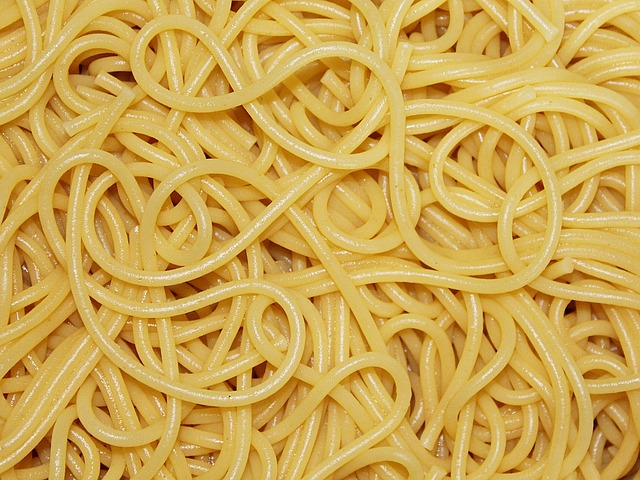
\includegraphics[width=.7\linewidth]{espaguetis}
\end{center}
\caption{Un plato de espaguetis sin estructurar}
\label{fig_pro}
\end{figure}

% Utilice «citet» para integrar el nombre del autor en el
% texto. Para referencias aisladas, «citep».

Durante la década de los sesenta, con el asentamiento del
concepto de la \emph{programación estructurada}, se fue
forjando un rechazo al recurso a esa intrucción de los
lenguajes de programación de alto nivel. En su célebre
carta, \citet{1968_Dijkstra} se declara convencido de que
«the go to statement should be abolished from all
  “higher level” programming languages (i.e. everything
  except—perhaps—plain machine code)». Ese \emph{perhaps}
parecía estar pidiendo innovaciones radicales en la
aquitectura de procesadores.

La propuesta de privación del recurso a los «gotos» no gozó
del asentimiento general: «Dijkstra once told me that he
actually received “a torrent of abusive letters” after
publication of his article» \citep[p. 265]{1974_Knuth}.

Sin embargo, a pesar de lo contundente de algunas
expresiones de la carta, no debería interpretarse esta,
seguramente, como una condena absoluta sobre los saltos
(\citet{1974_Knuth} reproduce estas palabras de Dijkstra:
«please don’t fall into the trap of believing that I am
terribly dogmatical about»), ni menos aún deducir que la
eliminación de los «gotos» es la fórmula mágica para lograr
un programa bien estructurado.

Knuth planteaba como objetivo la definición de uno o varios
juegos de estructuras, como el manejo de excepciones, para
ponerlas a disposición del programador. Auguraba un lenguaje
de programación consensuado para el año 1\,984: «Will
\textsc{Utopia 84} or, perhaps we should call it
\textsc{Newspeak}, contain {\bf go to} statements?».

Parece escéptico sobre su desaparición completa:
«... several languages have appeared in which the designers
proudly announced that they have abolished the \textbf{go
  to} statement. [...] which originally replaced \textbf{go
  to’s} by eight so-called “escape” statements. And the
eight weren’t even enough; the authors wrote, “Our mistake
was in assuming that there is no need for a label once the
\textbf{go to} is removed,” and they later [...] added a new
statement “\textbf{leave} $\langle$label$\rangle$
\textbf{with} $\langle$expression$\rangle$” which goes to
the place \emph{after} the statement identified by the
$\langle$label$\rangle$. Other \textbf{go to}-less languages
[...] and language designers still feel the need for some
euphemism that “goes to” without saying \textbf{go to}».

Añade: «... we shouldn’t merely remove \textbf{go to}
statements because it’s the fashionable thing to do; the
presence or absence of \textbf{go to} statements is not
really the issue. [...] undisciplined \textbf{go to}
statements make program structure harder to perceive, and
they are ofter symptoms of a poor conceptual
formulation». But there has been far too much emphasis on
\textbf{go to} elimination instead of the really important
issues; people have a natural tendency to set up an easily
understood quantitative goal like the abolition of jumps,
instead of working directly for a qualitative goal like a
good program structure» \citep{1974_Knuth}.

Si la controversia polarizada es ingrediente imprescindible
para el interés general, la respuesta de \citet{1987_Rubin}
abanderó la posición favorable a los «gotos», achacándole
dos faltas a la carta de Dijkstra: ser académica y poco
convincente. Según él, la identificación entre programación
estructurada y sin «gotos» es lo que «has caused
incalculable harm to the field of programming, which has
lost an efficacious tool». Se queja de que «some people have
devised program complexity metrics penalizing \textbf{GOTOs}
so heavily that any program with a \textbf{GOTO} is
\emph{ipso facto} rated more complex than even the clumsiest
\textbf{GOTO}-less program».

Rubin propone, para mostrar la utilidad del «goto», la tarea
de programar la búsqueda de la primera fila no nula de una
matriz cuadrada.

% Reproduce un fragmento de código.
\codigo[commandchars=\\\{\}]{codigo_04c.c}{con}{7.5cm}
\hfill
\codigo{codigo_01b.c}{sin}{7.5cm}

% Añadiendo la opción «commandchars=\\\{\}», los caracteres
% \, { y } del archivo fuente se interpretan como código
% LaTeX y puede darse formato al código (manualmente). Hay
% que tener esto en cuenta cuando estos caracteres formen
% parte del código en sí.
%
% Sin esa opción, el fichero de reproduce tal cual.

Sin encontrar satisfactorias las contestaciones que se
opusieron a la carta de Rubin \citep{1987_Moore},
\citet{1987_Dijkstra} vuelve a la carga. Imbuido tal vez del
ánimo de la dispu\-ta, entra a degüello, sin tolerarle a
Rubin una vacilación entre mayúsculas y minúsculas
siquiera. Rechaza, por ejempo, el uso de las construcciones
{\tt and} (y {\tt or}) condicionales, como las que aparecen
en la versión «sin».

Dijkstra está a otros menesteres y no le duelen prendas en
añadir variables: «a competent professional programmer [...]
should not waste his time in pointing out that the boolean
variable \texttt{d} is superfluous».

\begin{center}
% Puede pasar parámetros al comando «VerbatimInput» del
% paquete «fancyvrb». Por ejemplo:
\codigo[numbers=none,frame=single]{codigo_05b.py}{}{11.5cm}
\end{center}

En esta memoria procuraremos esclarecer el siguiente problema:

% Un recuadro sombreado:
\begin{tcolorbox}
\lipsum[11]
\end{tcolorbox}

\chapter{\emph{Text scanning}}


\citet{1972_Knuth} describen dos tipos de programa que no
«submit gracefully to the new prohibition». Al organizar la
lectura de marcadores textuales, \citet[p. 271]{1974_Knuth}
se topa con un ejemplo parecido al siguiente.

\begin{minipage}{.6\linewidth}
\begin{center}
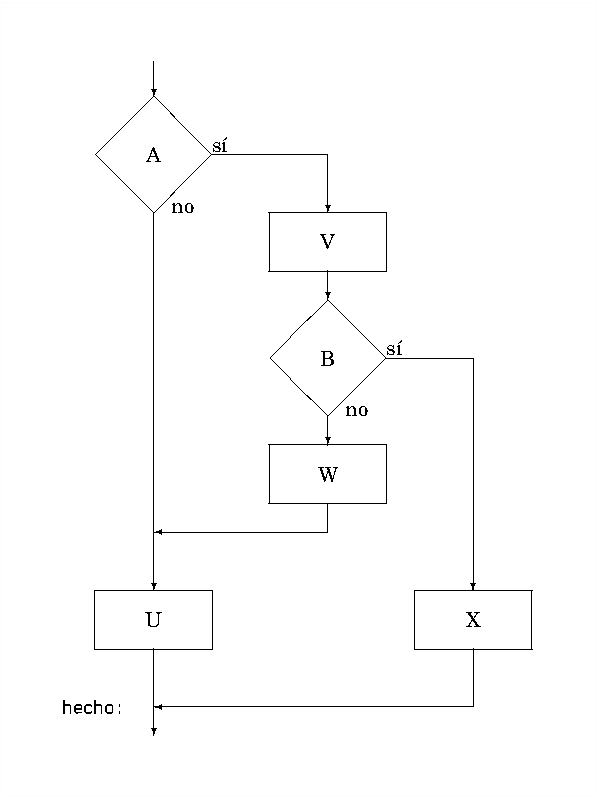
\includegraphics[scale=.8]{diagrama}
\end{center}
\end{minipage}
\hfill
\begin{minipage}{.3\linewidth}
\begin{center}
\NoCaptionOfAlgo
\begin{algorithm}[H]
\caption{con}
\SetKw{goto}{goto}
\DontPrintSemicolon
\If{A}{
  V\;
  \eIf{B}{
  X\;
  \goto \texttt{hecho}\;}{
  W\;}
}
U\;
\texttt{hecho:}
\end{algorithm}
\end{center}
\end{minipage}

¿Podríamos librarnos del «goto» sin duplicar código?

\NoCaptionOfAlgo
\begin{algorithm}[H]
\caption{sin}
\DontPrintSemicolon
\eIf{A}{
  V\;
  \eIf{B}{
    X\;}{
    W\;
    U\;
  }
}{
  U\;
}
\end{algorithm}
\vspace{5mm}

\lipsum[39-41]

\begin{figure}[ht!]
\begin{center}
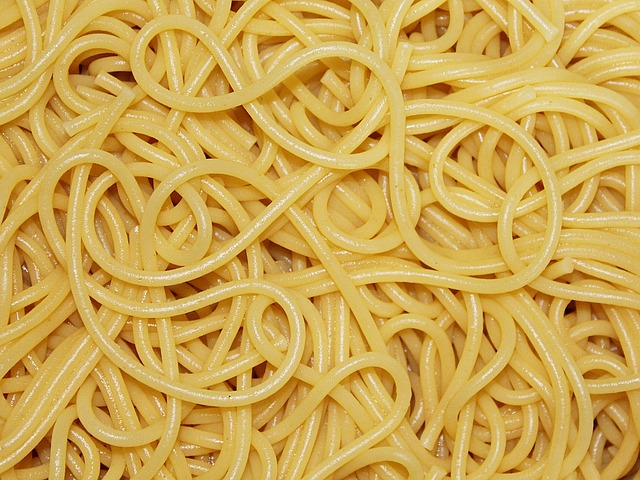
\includegraphics[width=\linewidth]{espaguetis}
\caption{}
\end{center}
\end{figure}

\lipsum[42-43]

\begin{figure}[ht!]
\begin{center}
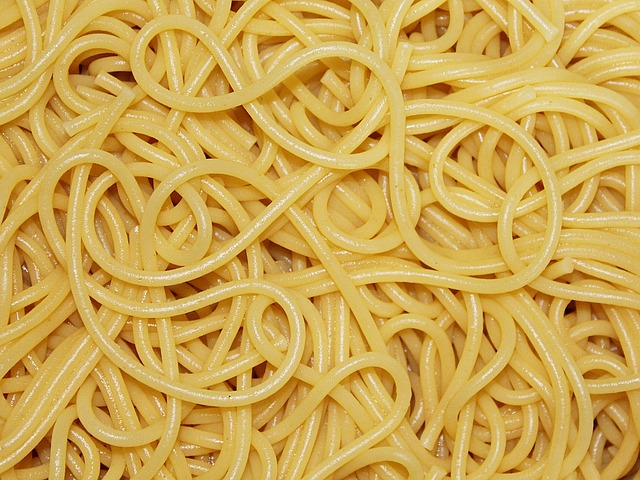
\includegraphics[width=\linewidth]{espaguetis}
\caption*{Sin número}
\end{center}
\end{figure}

\lipsum[45]

\input{capitulo3.tex}
\chapter{Conclusiones}

\lipsum[46-52]

\appendix
\chapter{Recuento de saltos}

\lipsum[1-24]



\backmatter
% Indique aquí el fichero .bib que contenga su bibliografía.
\bibliography{refs}

\end{document}
